%!TEX root = ../dissertation.tex

\section*{Thesis overview}

%!TEX root = ../dissertation.tex
\textbf{The relevance.} %of the research is determined by the low effectiveness of current software tools for inferring the model of the demographic history of populations from genetic data.
Metric tree models with functions on edges are used to analyze and predict various events of the real world, for example, processes represented as dynamic systems with variable structure~\cite{кириллов2009динамические, aldous1993continuum}.
\textit{Metric tree} is a graph that is a tree, where each edge is associated with an interval.
In general, metric graphs with functions on edges have found wide application, for example, in the form of quantum graphs~\cite{berkolaiko2013introduction}, which are used in physics in the study of quantum chaos~\cite{kottos1997quantum}, waveguides~\cite{exner2015quantum} and photonic crystals~\cite{kuchment2002differential}.

\textit{Model inferring} is a set of actions aimed at selecting the configuration, defining the model parameters and adjusting their values in order to achieve a high correspondence of the modeling results to the data of a full-scale experiment.
Expert data or assumptions about the object under study are usually required at various stages of model inferring.
These data may be inaccurate, limited or unknown, which can negatively affect the accuracy and adequacy of the model.
Automated construction methods allow to reduce the probability of human errors in model selection and parameters tuning.

When working with metric tree models with functions on edges, the participation of subject matter experts is resorted to.
Expert data is used to determine the properties of functions on the edges of the tree.
This information allows to establish the \textit{configuration} of the model, where each function on the tree belongs to a given family and is characterized by functional parameters available for tuning.
In the absence of expert data or in order to minimize the influence of the expert on the result, it is necessary to consider a set of all possible models differing in the types of functions and functional parameters.
For example, when building models of demographic histories for each population, piecewise-defined functions are considered consisting of functions of the three most popular types: constant, linear, and exponential.
Such an enumeration of configurations leads to an increase in the time required to infer the model.
The greater the number of allowed function types is, the more time will be required.
Additionally, it is required to keep track of the model complexity, the number of its parameters and overfitting.

Methods for tuning model parameters may also be limited in their degree of automation and require expert input.
For example, local search methods require the involvement of an expert to determine initial parameter values, and the effectiveness of the tuning depends on this choice.

Thus, when modeling real-world events in the form of a metric tree with functions on edges it is \textit{relevant} to develop specialized models and methods for automatic inference and tuning of models in order to minimize the influence of expert data on the result of modeling, which is considered in this dissertation on the example of the task of inferring demographic histories from genetic data.

A population is a group of individuals of the same species living in a specific area.
The \textit{demographic history of populations} is the history of populations' development and evolution, including events such as changes in population size, population splits, migration, and natural selection.
The reconstruction of the demographic history from genetic data is called \textit{demographic inference}.
Demographic histories are essential for dating historical events which have left no written records~\cite{goebel2008late, mellars2006going}, and they hold significance in fields such as conservation genetics \cite{nikolic2022stepping} and even medicine \cite{nielsen2007recent}.

Various statistical and algorithmic methods allow inference of demographic history models in the form of metric trees with functions on the edges and tuning their continuous parameters from genetic data.
In a case of demographic histories, the metric tree is the tree that defines the separation of populations, and the functions on the edges are the dynamics of population change.
As dynamics, we consider piecewise defined functions consisting of functions of the three most popular types: constant, linear, and exponential.
When building models, it is necessary to determine the number of time intervals, as well as the type of dynamics for each piecewise defined function.

Expert data is also involved at the stage of tuning the parameters of demographic history models, for which a combination of numerical simulation and optimization methods are used.
Numerical modeling methods are used to calculate the likelihood function, which allows estimating the degree of model fit to genetic data.
Local optimization methods are used to find the parameters that provide the maximum likelihood value.
It is these methods that are limited in the degree of automation: they require expert data to determine the initial values of parameters, and their efficiency depends on this choice.

The task of demographic inference is further complicated by the need for the user to implement the program code of the model and the algorithm for parameters' tuning.
Numerical modeling methods used by existing solutions have different capabilities and stability, and the user can apply several of them to compare the results.
However, when applying different software solutions simultaneously, the user is faced with the need to specify the same models using different interfaces.

Thus, the development of methods for automatic construction and tuning for models of metric trees with functions on edges will lead to minimizing the influence of expert data, and, consequently, to improving the quality of modeling of real-world events using real data from experiments.\\


% A population is a group of individuals of the same species living in a specific area.
% The \textit{demographic history of populations} is the history of populations' development and evolution, including events such as changes in population size, population splits, migration, and natural selection.
% By using various statistical and algorithmic methods, it is possible to reconstruct the demographic history from genetic data of individuals.
% This reconstruction is called \textit{demographic inference}.
% Demographic histories are essential for dating historical events which have left no written records~\cite{goebel2008late, mellars2006going}, and they hold significance in fields such as conservation genetics \cite{nikolic2022stepping} and even medicine \cite{nielsen2007recent}.
%
% In order to constrain the search space, existing methods for demographic inference usually involve the usage of demographic models --- parametric families of demographic histories.
%
% Currently, numerous methods and software tools provide means to specify a model of interest and to estimate model parameters from genetic data in order to obtain demographic history.
% These methods involve a combination of numerical modeling and optimization methods.
% They require a user (bioinformatician or systems biologist) to specify the model of the demographic history using the interface provided by the chosen software.
% Numerical modeling methods aim to compute the likelihood function of the demographic history and the data.
% The value of this function determines the optimality of the parameters and serves as the objective function in optimization algorithms.
% The vast majority of methods utilize local optimization algorithms to search for the parameters of the given model.
% These algorithms require the initial parameter values, and their effectiveness depends on this choice.

% Despite the availability of methods for demographic inference, the selection of models and the initial parameter values still require manual tuning and expert knowledge.
% As a result, it limits methods to obtain the best demographic history.
% In order to improve accuracy and reliability, users have to consider multiple models, find optimal parameters for each of them, and compare the results.
% The dynamics of population size change are always fixed in the considered models and, therefore, models primarily differ in values of these dynamics.
% Typically, three most popular dynamics are examined: constant population size, linear change, and exponential change.

% The problem of demographic inference is further complicated by the need for users to implement model code and parameter inference algorithms themselves.
% The numerical modeling methods used in existing solutions for likelihood evaluations have different capabilities and stability, and users may apply several methods to compare results.
% However, when using multiple software solutions simultaneously, users are faced with the obligation of specifying the same models using different interfaces.

% Therefore, the process of demographic inference requires significant time investment, especially when dealing with multiple populations.
% It also requires the user to have programming skills and knowledge about the studied biological species.
% These limitations restrict the capabilities of existing approaches for inferring demographic histories of populations and constructing models.\\

\textbf{State of the art.}
Graph models are studied and applied to solve a wide range of problems.
The works of A.M.~Raygorodsky~\cite{райгородский2010модели,райгородский2022модели} contain descriptions and examples of application of random graph models.
Graph-based probabilistic models such as Bayesian networks are extensively presented in the works of I.~Ben-Gal~\cite{ben2008bayesian} for modeling industrial systems~\cite{gruber2012efficient}, classification~\cite{gruber2019targeted}, or identification of transcription factor binding sites~\cite{ben2005identification}.
L.~Clark and D. Pregibon~\cite{clark2017tree} described examples of applications of tree-based models, which include, for example, decision trees~\cite{kotsiantis2013decision}.

The theory of metric graphs was formed by the works of V.G.~Boltiansky~\cite{болтянский1978комбинаторная}, P.S.~Soltan~\cite{soltan1973экстремальные,болтянский1978комбинаторная} and A.~Dress~\cite{dress1984trees}.
The properties of metric trees and the metric spaces generated by them have been studied by A.~Dress~\cite{dress1984trees}, B.~Buneman~\cite{buneman1974note} and D.~Aldous~\cite{aldous1991continuum_i,aldous1991continuum,aldous1991continuum,aldous1993continuum}.
In the works of A.S.~Matveev and S.I.~Matveev~\cite{матвеев2010создание,лёвин2011системы,матвеев2013интеллектуальная} metric graphs were applied in the construction of coordination models for intelligent navigation.

The development of models approximating implicit functions is also actively pursued by many scientists.
The most widespread application, described in the works of L.~Fahrmeir~\cite{fahrmeir2013regression} and R.~Snee~\cite{snee1977validation}, these models have received for solving regression problems.
When using piecewise-determined function models, the general form of the result functions is usually fixed, such as constructing piecewise-constant~\cite{schiffels2020msmc,dai2008nonlinear}, piecewise-linear~\cite{leenaerts2013piecewise}, or piecewise-exponential~\cite{friedman1982piecewise} models.
The number of function breakpoints as well as their positions are unknown characteristics of piecewise-defined function models.
In~\cite{muggeo2020selecting,malash2010piecewise}, methods for automatic model inference are presented to solve a piecewise-exponential regression problem, where the number of function breakpoints is determined using Bayesian information criterion (BIC) and Akaike information criterion (AIC)~\cite{akaike1974new}, respectively.

Models of metric trees with functions on graphs are a combination of metric tree models and functional models on edges.
Quantum graphs that are metric graphs with differential operators on edges and their applications are discussed in detail in the works of G.~Berkolaiko~\cite{berkolaiko2006quantum,berkolaiko2013introduction}.
Metric trees with functions on edges are used to model demographic histories of populations in the works of R.~Gutenkunst~\cite{gutenkunst2009inferring}, J.~Kamm~\cite{kamm2020efficiently}, A.~Ragsdale and S.~Gravel~\cite{ragsdale2019models, ragsdale2020unbiased}.
However, the methods presented in these works assume that the user defines and fixes the general form of the piecewise-defined function on the edges of the tree, and sets the initial values of model parameters for tuning procedure that use local optimization methods.
The works of D.~Portik~\cite{portik2017evaluating, leache2019exploring} and R.~Gutenkunst~\cite{blischak2020inferring} presented global optimization methods for parameter tuning of population history models that minimize but still require user involvement.
A general application of numerical optimization methods for different problems is presented in the classic paper by B.T. Polyak~\cite{поляк1983введение}, and a description of modern global optimization methods can be found in~\cite{пантелеев2013методы}.

At the time the author began his research (in 2017), there was no method for automatic model inference and tuning for metric tree models with functions on edges.
By the end of the dissertation research, the first alternative solution for a method for automatic model selection emerged, applied for the demographic inference problem~\cite{rippe2021environmental}.
However, the method allows analyzing models defined in a specific catalog and only for inferring demographic histories of \emph{two} populations.
Furthermore, the selection of the best model is made under the assumption of data independence, which is not always correct.\\

% The foundation of the demographic inference was built by the Japanese biologist M.~Kimura in his works in 1962~\cite{kimura1962probability, kimura1964diffusion} and 1969~\cite{ohta1969linkage}, as well as by scientists W.~Hill and A.~Robertson in their works in 1966~\cite{hill1966effect} and 1968~\cite{hill1968linkage}.
% However, it was only with the development of sequencing techniques and the accumulation of genetic data that these methods began to be actively utilized.
% Methods to infer specific characteristics of the demographic histories, for example, population growth rates~\cite{kuhner1998maximum}, were developed in the late 20th century.

% Methods for demographic inference of complex models with greater number of parameters appeared in the early 21st century.
% They were based on the idea of finding parameter values that maximize the likelihood function for the observed data.
% However, the development was focused mainly on methods for likelihood computation, while optimization was left to classical local search algorithms implemented in popular publicly available libraries such as SciPy~\cite{virtanen2020scipy}.
% The libraries \dadi~\cite{gutenkunst2009inferring}, \momi~\cite{kamm2020efficiently}, \moments~\cite{jouganous2017inferring}, and \momentsLD~\cite{ragsdale2019models, ragsdale2020unbiased} are among the most popular software tools for demographic inference.
% The \dadi library implements the diffusion approximation method for likelihood computation, \moments  and \momentsLD libraries employ the method of moments.
% All of these methods are based on numerical modeling.
% The popular libraries for parameter inference of complex demographic history models are presented in Table~\ref{tab:synopsis:list_dem_methods}.

% It is worth noting that the complexity of likelihood computation methods scales with the number of analyzed populations.
% As a result, some software tools only support a limited number of populations for the analysis.
% For example, \dadi and \moments have a complexity of likelihood computation methods that scales exponentially, and they can only analyze up to three and five populations, respectively.

% \begin{table}[ht]
%     \centering
%     \resizebox{\linewidth}{!}{%
%     \begin{tabular}{|l|l|l|l|l|l|l|}
%         \hline
%         Software & Year & Interface &  Likelihood & Optimization        & Requirement & Supported \\
%             &     & for model &   evaluation  & methods  & of the initial & number of \\
%                    &     & specification & method &              &                  parameters & populations \\
                   
%         \hline
%         \dadi   & 2009  & Yes & Diffusion & Four local & Yes & Up to three \\
%                 &       & (models & approximation    & search methods & & \\
%                 &       &  of I class) &              & plus one global      & & \\
%                 &       & &              & search method     & & \\
%                 &       & &              & (2020)     & & \\
%         \hline
%         \moments& 2017  & Yes & Moment closure& Four local &  Yes & Up to five \\
%                 &      & (models & method for allele  & search methods  & & \\
%                 &   &  of I class) & counts statistic &      & & \\
%         \hline
%         \momentsLD& 2019 & Yes & Moment closure & Four local & Yes & Any \\
%                 &       &  (models & method for linkage & search methods  & & \\
%                 &      & of I class) & disequlibrium &       & & \\
%                 &      & & statistic &       & & \\
%         \hline
%         \momi   & 2020  & Yes & Continuous    & One method & Yes & Any \\
%                 &   & (models    & Moran model  & truncated & & \\
%                 &   &   of II class) &                & Newton & & \\
%                 &    &   &                & method       & & \\
%         \hline
%         \textit{dadi-pipeline}   & 2017  & No & Method   & One method of & No & Up to three \\
%                 &   & (interface    & from \dadi  & multiple rounds of& &\\
%                 &   &  of \dadi) &                & Nelder-Mead & & \\
%                 &    &    &                &  method       & & \\
%         \hline
%         \textit{moments-pipeline}   & 2019  & No & Method   & One method of & No & Up to five \\
%                 &   & (interface     & from \moments  & multiple rounds of & &\\
%                 &   &  of \moments) &                & Nelder-Mead & & \\
%                 &    &    &                & method      & & \\
%         \hline

% %        \textit{fastsimcoal2} & 2013 
% %          & Симуляция    & 1 алгоритм  & до $\infty$ &  Да & Да\\
% %        & & процесса     & ECM-алгоритм & & & \\
% %        & & коалисценции & (Expectation & & & \\
% %        & &              & Conditional & & & \\
% %        & &              & Maximization) & & & \\
% %        \hline
%     \end{tabular}%
%     }
%     \caption{Existing software tools for demographic inference from genetic data}
%     \labelsyn{tab:synopsis:list_dem_methods}
% \end{table}

% There was no method available for demographic inference without a predefined model configuration at the time the research was started (in 2017).
% Additionally, there was a lack of global optimization methods for efficient search of the maximum-likelihood model parameters.
% All existing solutions required researchers to specify the model and provide the initial parameters' estimates for local search optimization algorithms.
% It posed challenges for the main audience of these software tools and led to usage errors.
% Furthermore, searching for model parameters for a large  populations' counts, like four and five populations in the \moments library, was computationally demanding.

% D.~Portik introduced the software tools \textit{dadi pipeline} and \textit{moments pipeline} as wrappers for the \dadi and \moments libraries, respectively, in 2017 and 2019~\cite{portik2017evaluating, leache2019exploring}.
% These tools provide a catalog of implemented models for the user to choose from, which eliminates the need for manual model specifications and reduces the probability of errors.
% Moreover, \textit{dadi pipeline} and \textit{moments pipeline} implement a global search algorithm that sequentially executes multiple rounds of Nelder-Mead local optimization.
% In order to address the issue of initial parameter selection, the authors proposed the usage of common parameter values across all models and the noise application to parameters before each optimization round.
% Thus, the proposed method has several hyperparameters, including the number of local search rounds and the noise level applied to the parameters.
% It is important to note that the optimal values of these hyperparameters, required to achieve global optima, were not determined and are left to the user's choice.

% % The first publication of the author~\cite{noskova2020gadma} in 2020 addressed the inefficiency of existing optimizations and the lack of a method for automatic model selection.
% % The class of extended models, a genetic algorithm for parameter tuning, and a method for automatic model selection described in this thesis were presented in the paper.
% % After the preliminary non-peer-reviewed publication of this article and its submission to a journal in 2019, the authors of the \dadi library incorporated the BOBYQA global search algorithm~\cite{powell2009bobyqa} into the library.
% % However, it still requires the initial parameters to be set by users~\cite{blischak2020inferring}.

% % The alternative solution for the automatic model selection of the demographic history for \emph{two} populations was presented~\cite{rippe2021environmental} a year after the publication of the author's article~\cite{noskova2020gadma}.
% % The presented software is a wrapper for \moments and contains a large catalog of more than 100 models for parameters tuning, and comparison.
% % The selection of the best model assumes data independence, which is not always valid.
% % The latest version of this software tool uses a genetic algorithm developed in this work as the optimization method.

% % The emergence of new methods for model selection and optimization, as well as the active use of the methods developed by the author, demonstrates the increased interest in the problem addressed in this work, making it highly relevant.\\

% By the end of the dissertation research, the authors of the \dadi library incorporated the BOBYQA global search algorithm~\cite{powell2009bobyqa} into the library.
% However, it still requires the initial parameters to be set by users~\cite{blischak2020inferring}.
% Moreover, the alternative solution to the automatic demographic model selection method presented in this study was introduced~\cite{rippe2021environmental}.
% However, the proposed software allows analyzing data for only \emph{two} populations using \moments.
% The selection of the best model assumes data independence, which is not always valid.
% The latest version of this software tool uses a genetic algorithm developed in this work as the optimization method.\\

The \textbf{aim} of this thesis is to improve the quality of computer modeling of real-world events by developing methods, and software packages for automatic inference and tuning of metric tree models with functions on edges.\\

In order to achieve this aim, the following \textbf{tasks} have been defined and completed:
\begin{itemize}
    \item investigate the current state of the subject area, refine the problem, and determine methods for evaluating the results;
    \item formalize the problem of model inferring and tuning for metric tree models with functions on edges;
    \item develop a method for automatic tuning of metric tree models with functions on edges based on a combination of global and local optimization methods;
    \item develop a method for automatic selection of metric tree models with piecewise defined functions on edges;
    \item design and implement a software framework that incorporates the developed models and methods for inferring the demographic history of populations from genetic data;
    \item conduct experimental studies confirming the effectiveness of the developed models and methods, as well as their applicability for inferring the demographic history of populations from genetic data, analyze the results of experiments.\\
\end{itemize}

The \textbf{scientific novelty} of the thesis is as follows:
%(1) a class of extended models that includes models with discrete parameters for population size dynamics is developed;
(1) methods based on a combination of global and local optimization techniques for parameter tuning of a given metric tree model with functions on edges are developed;
(2) method for automatic selection of metric tree model with piecewise-defined functions on edges that does not require expert involvement is developed.\\
%(4) new population demographic histories that provide a better likelihood values compared to previous results obtained using local search methods and expert participation are derived for the subject area.\\

The \textbf{theoretical significance} of the thesis lies in = extension of the classical formulation of the problem of tuning a metric tree model with functions on edges not only as a problem of tuning the parameters of a given model, but also as a problem of selecting the model itself automatically.
The obtained modeling and tuning methods are applicable to arbitrary metric tree models with functions on edges.
Moreover, the developed optimization methods can be used or adapted for optimization problems in other scientific fields.\\

The \textbf{practical significance} of the thesis is determined by:
\begin{itemize}
    \item the extension of the scientific and practical toolkit of bioinformaticians with methods and algorithms for demographic inference;
    \item the open-access source code of the developed software framework GADMA, which is available for reuse at the following address: \url{https://github.com/ctlab/GADMA};
    \item the applicability of the developed methods for the analysis of genetic data;
    \item incorporation of the developed method based on a genetic algorithm into a third-party software~\cite{rippe2021environmental}.\\
\end{itemize}

\newpage
\textbf{Principal statements of the thesis:}
\begin{enumerate}[label={\arabic*.}]
    \item The method of modeling and parameter tuning of metric tree models with functions on edges based on field experiment data, that contains models with continuous functional parameters, characterized in that for the purpose of automatic tuning without involving expert data it uses models with discrete parameters that define families of functions, as well as global optimization methods --- genetic algorithm and Bayesian optimization, and a set of programs implementing it.
    \item The method of automatic selection of metric tree model with functions on edges with different number of parameters and tuning of these parameters basen on field experiment data, that contains the Akaike information criterion for model comparison, characterized in that in order to increase the level of automatization and to provide an opportunity to tune not only the model parameters, but also the model itself, it includes a method of increasing the number of time intervals for piecewise-defined functions on edges of a tree, as well as a set of programs implementing it.
\end{enumerate}

\textbf{Research methods.} The study utilized optimization methods, numerical methods, probability theory and mathematical statistics, machine learning techniques, and methods for conducting experimental research.\\

\textbf{Soundness and correctness} of scientific results obtained in this thesis are ensured by the correct utilization of methods, the formulation of well-justified problem statements, and the extensive experimental investigations that cover the developed technologies and algorithms.
The population demographic histories obtained with the developed methods on verified simulated data are consistent with the original histories used for modeling.
The results obtained from real data align with previously published studies~\cite{gutenkunst2009inferring, jouganous2017inferring, nielsen2017tracing, verissimo2017world, king2015genetic, сивцева2020геном}.\\

\textbf{Compliance with specialty requirements.}
In accordance with the specialty passport 1.2.2 --- «Mathematical modeling, numerical methods, and software frameworks (computer science)» the dissertation belongs to the following fields of research:

\textbf{Point 2 of the specialty passport} «Development, justification, and testing of efficient computational methods using modern computer technologies».
Methods for tuning the parameters of metric tree models with functions on edges based on numerical optimization methods were developed, justified and tested.

\textbf{Point 4 of the specialty passport} «Development of new mathematical methods and algorithms for interpretation of natural experiment on the basis of its mathematical model».
This dissertation study presents methods for building metric tree models with functions on edges from natural experiment data in order to analyze real world events.\\

% \textbf{Point 9 of the specialty passport} «Setting up and conducting computational experiments, statistical analysis of their results, including with the use of modern computer technologies (computer sciences)».
% The development of the GADMA software package allowed to conduct many computational experiments to infer demographic histories from genetic data.
% The results of the computational experiments are analyzed, and different models are compared using statistical methods such as Akaike's information criterion and likelihood ratio test.\\

\newpage
\textbf{Dissemination.}
The main results of the thesis were presented at the following conferences:

\begin{itemize}
    \item International Congress «VII Congress of the Vavilov Society of Geneticists and Breeders dedicated to the 100th anniversary of the Department of Genetics, SPbSU, and associated symposia», 2019, St. Petersburg, Russia;
    \item Moscow Conference on Computational Molecular Biology, 2019, Moscow, Russia;
    \item Probabilistic Modeling in Genomics, 2019, Aussois, France;
    \item Probabilistic Modeling in Genomics, 2021, virtual;
    \item Moscow Conference on Computational Molecular Biology, 2021, Moscow, Russia;
    \item Probabilistic Techniques in Analysis: Spaces of Holomorphic Functions, 2021, Sochi, Russia;
    \item LI Scientific and educational conference of ITMO University, 2022, ITMO University, St. Petersburg, Russia;
    \item Probabilistic Modeling in Genomics, 2022, Oxford, UK;
    \item The XI Congress of Young Scientists, 2022, ITMO University, St. Petersburg, Russia;
    \item Conservation Genomics at the Population Level, 2022, Cambridge, UK;
    \item Probabilistic Modeling in Genomics, 2023, Cold Spring Harbor, NY, USA;   
    \item The XII Congress of Young Scientists, 2023, ITMO University, St. Petersburg, Russia;
    \item  Society for Molecular Biology and Evolution Meeting (SMBE23), 2023, Ferrara, Italy.\\
\end{itemize}

\textbf{Awards} 
\begin{itemize}
    \item Bronze Award in the 17th Human-Competitive Awards category at the Genetic and Evolutionary Computation Conference (GECCO) virtual conference in 2020.
    \item Winner of the System Biology Fellowship from Skolkovo Institute of Science and Technology for the project «Computational methods for unsupervised demographic inference of multiple populations from genomic data» in 2021. The number of winners is five per country per year.\\
\end{itemize}

\textbf{Publications}

Based on the results presented in the thesis, eight articles were published in peer-reviewed scientific journals included in the international abstract databases and citation systems Scopus and Web of Science.\\


\textbf{Personal contribution}

\begin{enumerate}[label=\arabic*.]
    \item 
    In the publication~\cite{noskova2020gadma} Noskova E. --- development and implementation of genetic algorithm and method for automatic selection of demographic history model from genetic data, conduction of the experimental studies (80\%); Ulyantsev~V. --- supervision on problem formulation, selection, and justification of theoretical foundations of scientific research (10\%); Koepfli~K.P., O'Brien~S.J. --- advice in conducting experimental studies and writing a paper (5\%); Dobrynin~P. --- supervision on problem formulation (5\%).

    \item %\cite{noskova2022gadma2}: 
    In the publication~\cite{noskova2023gadma2} Noskova E. --- development and implementation of methods, software for demographic inference from genetic data, conduction of the experimental studies (85\%); Abramov~N., Iliutkin~S., Sidorin~A. --- software development (10\%); Dobrynin~P., Ulyantsev~V. --- supervision on problem formulation, selection, and justification of theoretical foundations of scientific research (5\%).

    \item %\cite{noskova2022bayesian}: 
    In the publication~\cite{noskova2023bayesian} Noskova E. --- development and implementation of the Bayesian optimization method for demographic inference from genetic data, conduction of the experimental studies (90\%); Borovitskiy~V. --- recommendations on problem formulation, selection, and justification of theoretical foundations of scientific research (10\%).

    \item %\cite{zhernakova2020genome}: 
    In the publication~\cite{zhernakova2020genome} Noskova E. --- demographic inference of the history of three  modern human populations (10\%); Ulyantsev~V. --- supervision (5\%); other co-authors --- collection and analysis of the genetic data (85\%).

    \item %\cite{nikolic2022stepping}: 
    In the publication~\cite{nikolic2022stepping} Noskova E. --- demographic inference of the history of two and three populations of blue sharks (10\%); the other co-authors --- collection and analysis of the genetic data (90\%).

    \item %\cite{adrion2020community}: 
    In the publication~\cite{adrion2020community} Noskova E. --- software development and testing of the genetic data simulations (5\%); other co-authors --- software development, testing, and conduction of the experimental studies (95\%).

    \item %\cite{lauterbur2023expanding}: 
    In the publication~\cite{lauterbur2023expanding} Noskova E. --- implementation of published demographic histories in the software for genetic data simulations (5\%); other co-authors --- software development (95\%).
    
    \item %\cite{gower2022demes}: 
    In the publication~\cite{gower2022demes} Noskova E. --- software development for the representation of the demographic histories (5\%); other co-authors --- software development (95\%).\\.
\end{enumerate}


\textbf{Scope and structure of the work}

% The dissertation consists of an introduction, four chapters, a conclusion, and an appendix.
% The full length of the dissertation is
% \formbytotal{TotPages}{pages}{}{}{}, including
% \formbytotal{totalcount@figure}{figures}{}{}{},
% \formbytotal{totalcount@table}{tables}{}{}{}, and eight listings.
The dissertation consists of an introduction, four chapters, a conclusion, and an appendix.
The full length of the dissertation is 396 pages, including
120 figures, 16 tables and eight listings.
The list of references contains 171 references.

\newpage
\section*{Thesis contents}

The relevance of the scientific research conducted within the framework of this dissertation is justified in the \textbf{introduction}.
The state of the art of the demographic inference from genetic data is described, and an overview of the methods for modeling demographic histories is provided.
The goals and objectives of the research are formulated, and the scientific novelty, theoretical significance, and practical implications of the work are described.
Additionally, the principal statements of the thesis are listed.

The \underline{\textbf{first chapter}} presents a comprehensive overview of the subject area.
It includes the definition of the demographic history of populations and the description of the existing methods for inferring demographic histories from genetic data.

The fundamental definitions in population genetics used in this dissertation are described in \textbf{Section 1.1}.
Population genetics is an important field within genetics that investigates the changes in the genetic composition of populations and their evolution.
It addresses various tasks such as determining population structure, constructing phylogenetic trees, and inferring the demographic history of populations.
The section begins with the formal definition of the demographic history of populations.

\emph{Demographic history of populations} refers to the populations' history of evolution and development.
It includes information about population splits, population size changes, migration rates, \textit{inbreeding coefficients} (the degree of consanguineous relationships), and more.
Examples of visual representations of demographic histories are shown in Figure~\ref{fig:syn_rus:dem_inf:dem_his_examples}. 
The colored areas demonstrate how populations split --- the population tree.
Information about population size is depicted by the width of those areas, and arrows between them represent migrations.
Time in demographic histories is often measured in generations or years and is represented along the y-axis.

\begin{figure}[b]
    \centering
    \begin{subfigure}[b]{.33\textwidth}
    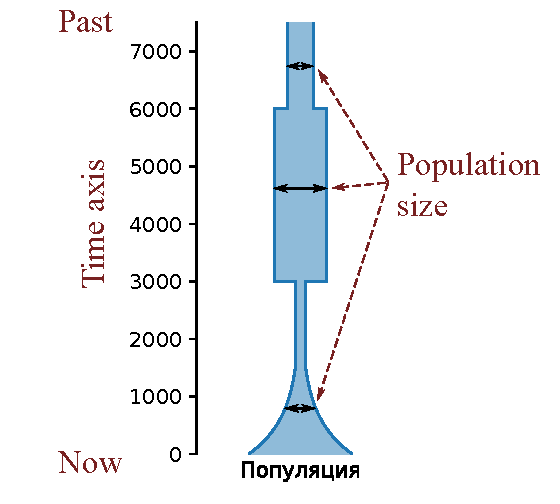
\includegraphics[width=\textwidth]{images/part1/dem_history/1d_model_fixed_en.pdf}
    \caption{}
    \labelsyn{fig:syn_rus:dem_inf:dem_his_examples_1}
    \end{subfigure}%
    \begin{subfigure}[b]{.33\textwidth}
    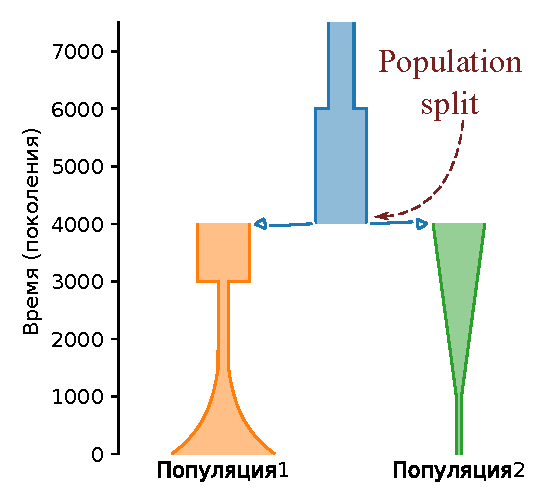
\includegraphics[width=\textwidth]{images/part1/dem_history/2d_model_isolation_fixed_en.pdf}
    \caption{}
    \labelsyn{fig:syn_rus:dem_inf:dem_his_examples_2}
    \end{subfigure}%
    \begin{subfigure}[b]{.33\textwidth}
    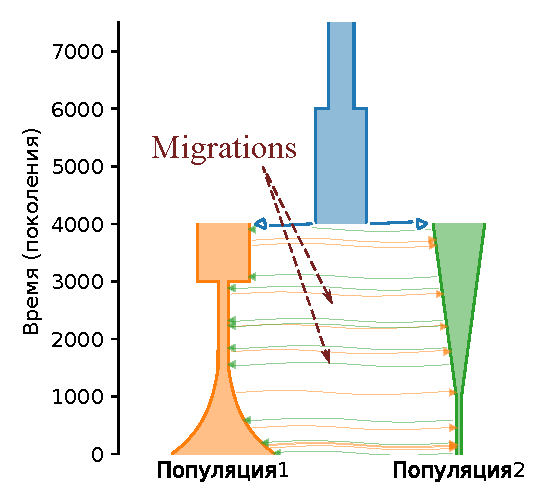
\includegraphics[width=\textwidth]{images/part1/dem_history/2d_model_migration_fixed_en.pdf}
    \caption{}
    \labelsyn{fig:syn_rus:dem_inf:dem_his_examples_3}
    \end{subfigure}
    \caption{Examples of visual representations of the demographic histories of one and two populations}
    \labelsyn{fig:syn_rus:dem_inf:dem_his_examples}
\end{figure}


%\newpage

\textit{Demographic inference} is the reconstruction of the demographic history from genetic data.
The problem of demographic inference and its solutions are described in \textbf{Section 1.2}.
The existing solutions aim to find demographic history using parametric models.
The section includes the description of the main methods and components of existing methods for demographic inference.
A brief description of well-known software tools implementing these methods, namely \dadi, \moments, \momi, and \momentsLD, is also provided.

Parametric models are used for searching demographic histories of populations.
These models are metric trees with functions defined on edges.
Models usage allows constraining the search space and tuning the model parameters using optimization methods.
Figure~\ref{fig:model_def2} shows a model example in the form of metric tree with functions on edges that describes the demographic history of two populations.

\begin{figure}[ht]
    \centering
    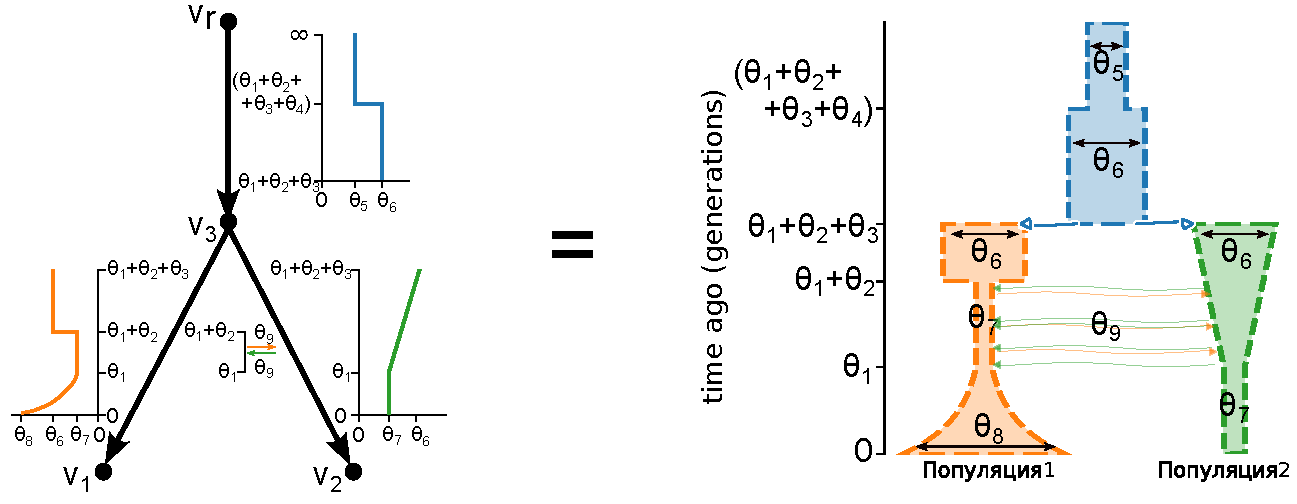
\includegraphics[width=0.8\textwidth]{images/part1/2d_model_metric_tree_2.pdf}
    \caption{Example of the model of demographic history of two populations in the form of a metric tree with functions on edges}
    \labelsyn{fig:model_def2}
\end{figure}

The problem of inferring the demographic history of populations from genetic data involves \textit{parameter tuning} of a given parametric model, i.e. finding model parameters that maximize the likelihood function of the genetic data (Figure~\ref{fig:part1:deminf:general_scheme}).
Existing software solutions differ in their model specification interfaces, likelihood computation methods, and parameter optimization methods.

\begin{figure}[ht]
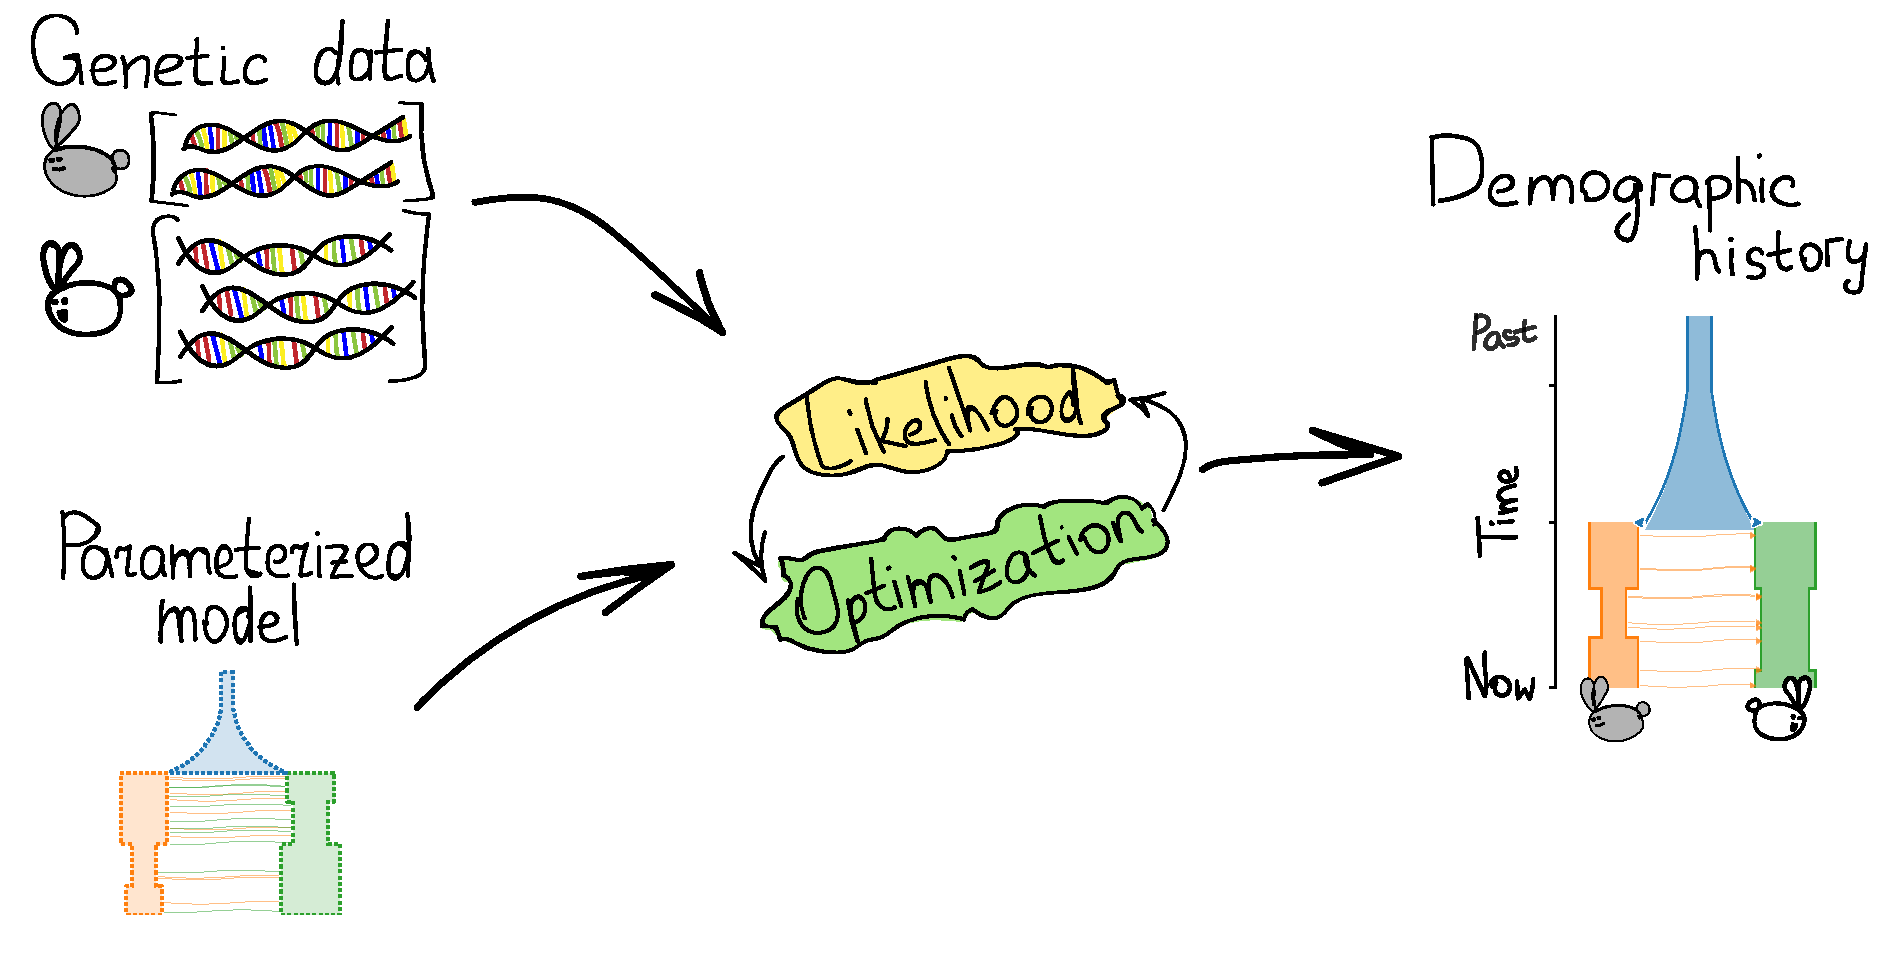
\includegraphics[width=0.7\textwidth]{images/part1/dem_history/general_scheme_en.pdf}
\caption{Example input and output of existing software solutions for the demographic history inference from genetic data}
\labelsyn{fig:part1:deminf:general_scheme}
\end{figure}

Two classes of demographic history models used in existing solutions are described in \textbf{Section 1.3}, along with methods for comparing models with different numbers of parameters.

\textit{Models of the first class} are used in the software solutions \dadi, \moments, and \momentsLD.
They are represented as a sequence of elements corresponding to time intervals, population splits, pulse migrations, and inbreeding events (Figure~\ref{fig:dadi:model_spec}).
These models have only continuous parameters, and the dynamics of population size (constant, linear, or exponential) are fixed within these models.

\begin{figure}[b]
\centering
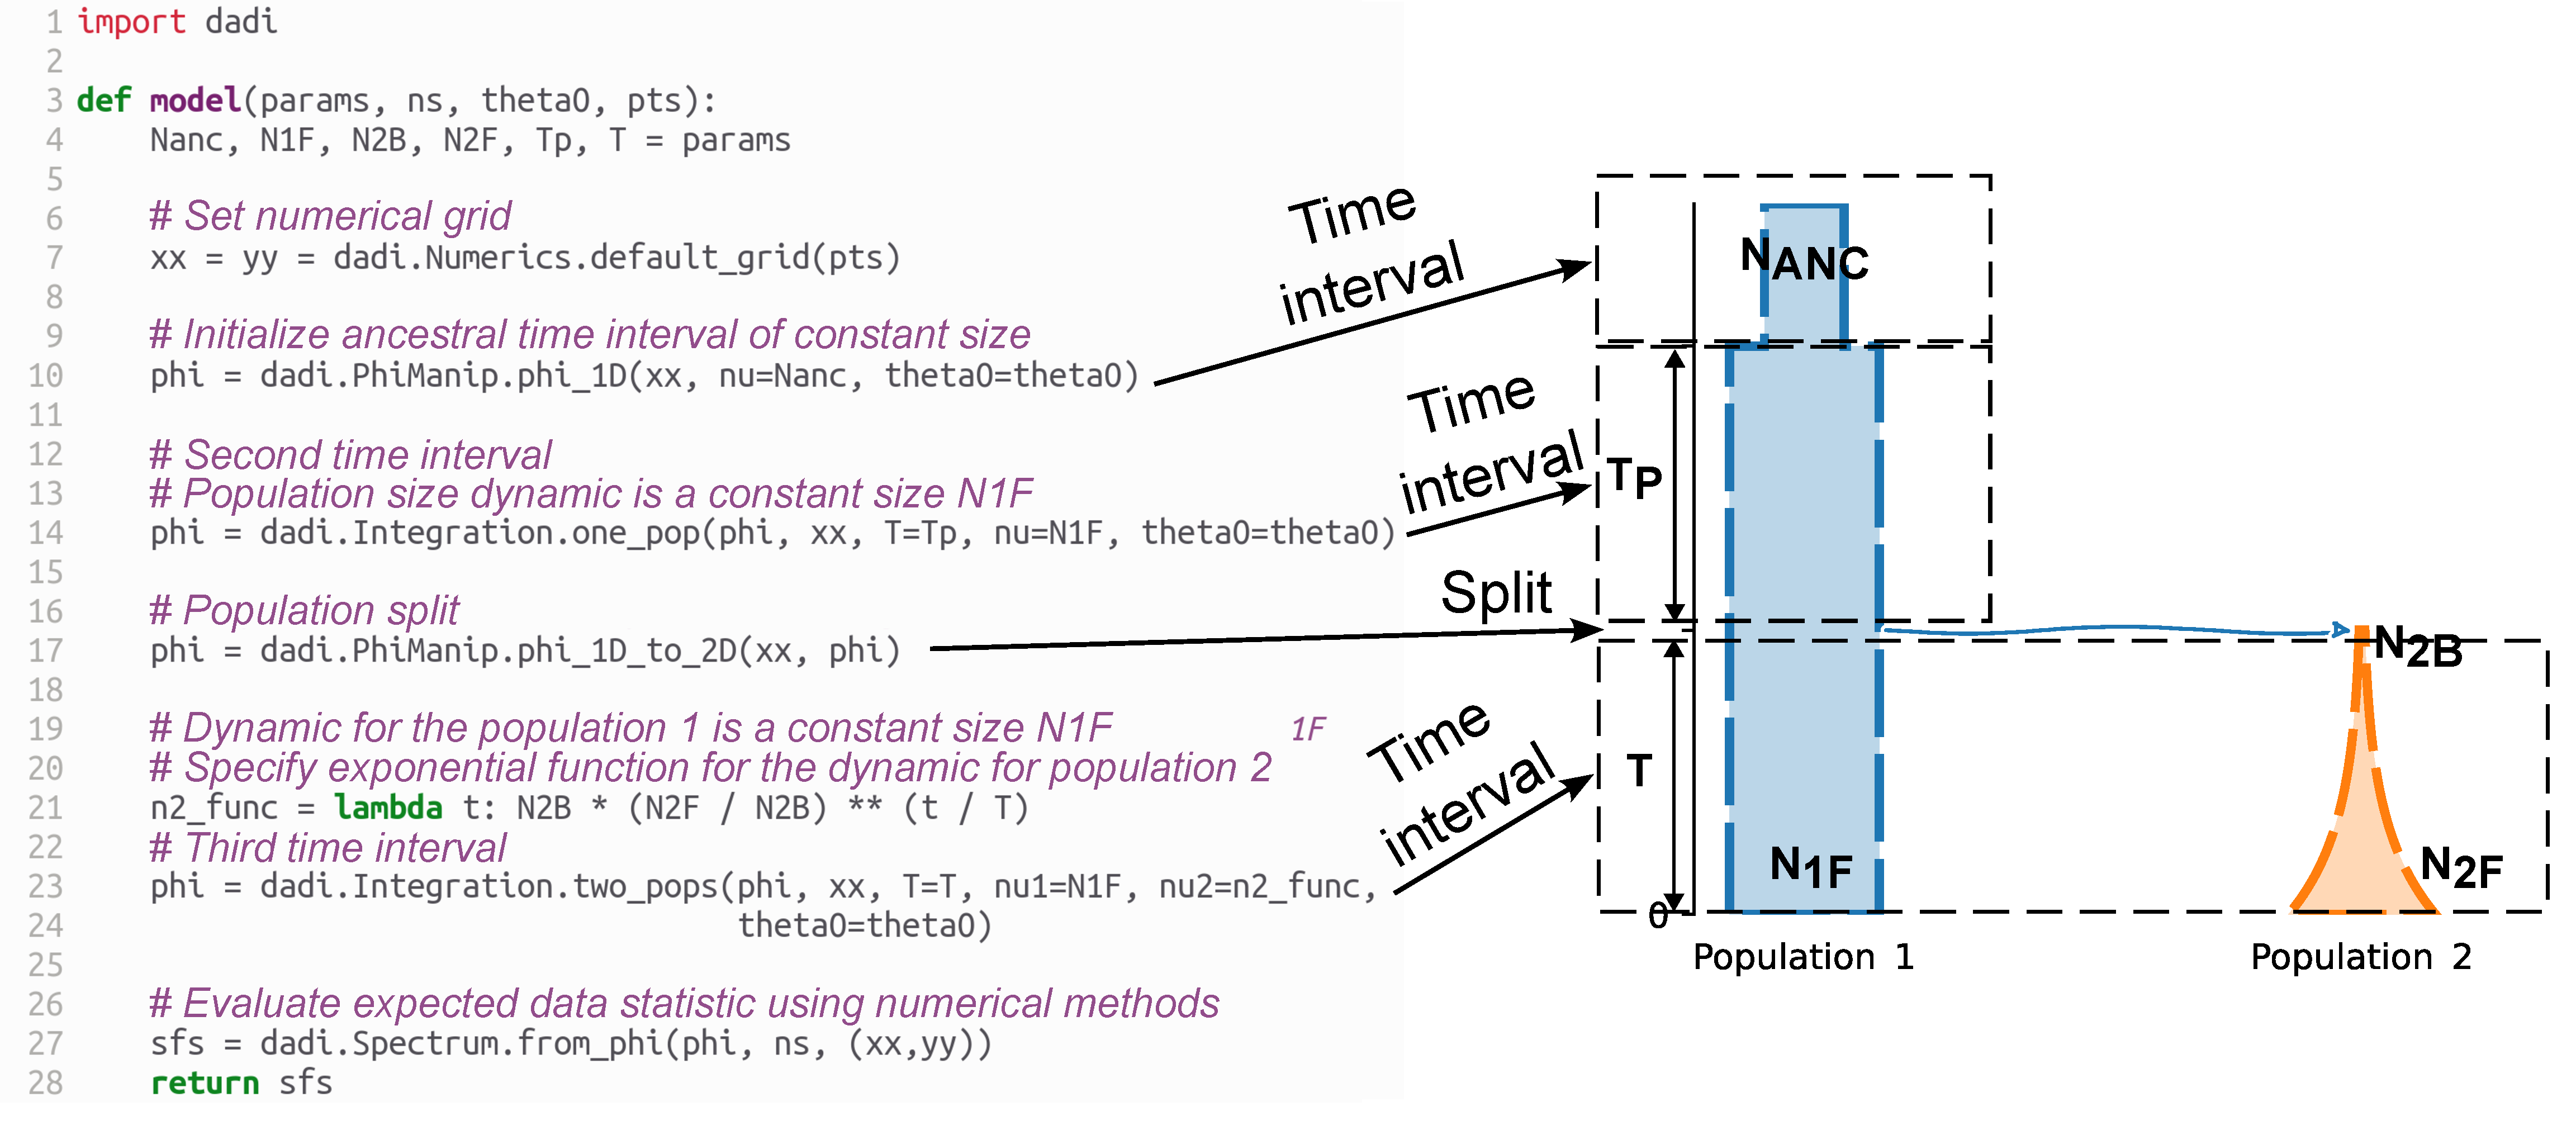
\includegraphics[width=\linewidth]{images_2/dadi_model_en.pdf}
\caption{Example specification of the first class model using the \dadi library interface}
\labelsyn{fig:dadi:model_spec}
\end{figure}

\textit{Models of the second class} are used in the software solution \momi.
They are represented as a set of events related to changes in population size, population splits, and single migrations.
Models of the second class also have only continuous parameters and fixed dynamics of population size.
However, they are more limited compared to models of the first class, for example, they do not support linear population size changes or continuous migrations.

The model selection problem is generally stated as follows: choose the model that is most suitable for the data.
A simple model with a small number of parameters may not reflect some information in the data.
On contrary, the complex model with a large number of parameters may overfit to noise in the data and ultimately model the underlying process incorrectly.
To compare different models and choose the best one, the Akaike information criterion (AIC)\cite{akaike1974new}, Bayesian information criterion (BIC)\cite{schwarz1978estimating}, and likelihood ratio test~\cite{vuong1989likelihood} are commonly used.

An overview of existing methods for computing the likelihood of genetic data given a specified demographic history is provided in \textbf{Section 1.4}.
The section includes definitions of key biological and genetic concepts, such as DNA, genes, alleles, and genotypes.
The main data statistics are described, including the allele frequency spectrum and statistics based on linkage disequilibrium.
Finally, the methods for likelihood evaluation implemented in the software solutions \dadi, \moments, \momi, and \momentsLD are described.

In \textbf{Section 1.5}, a general description of local and global optimization methods is provided, highlighting the key differences between these two groups, along with an overview of existing optimization methods for parameter tuning in demographic history models using genetic data.
Principally, local optimization methods such as the Broyden-Fletcher-Goldfarb-Shanno (BFGS) method~\cite{broyden1970convergence, fletcher1970new, goldfarb1970family, shanno1970conditioning}, the Nelder-Mead method~\cite{nelder1965simplex}, and the Powell method~\cite{powell1964efficient} are employed for demographic inference (Figure~\ref{fig:syn_ru:opt:opt_example}).
Existing optimization methods for parameter tuning in models are limited to inference of continuous parameters only and require user involvement to specify initial model parameter and method hyperparameters, such as the number of restarts.
The use of local optimization methods does not guarantee finding the global optimum.

\begin{figure}[hb]
\begin{subfigure}[b]{\linewidth}
\centering
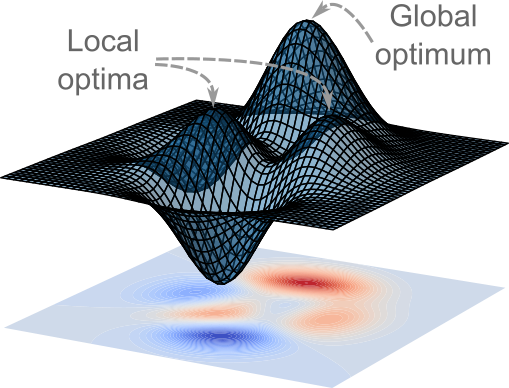
\includegraphics[height=3.2cm]{images/part1/opt/example_3d_en.png}
\caption{}
\labelsyn{fig:syn_ru:opt:opt_example_3d}
\end{subfigure}
\begin{subfigure}[b]{.33\linewidth}
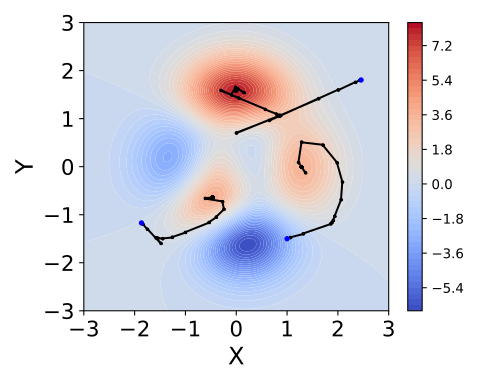
\includegraphics[height=3.2cm]{images/part1/opt/example_bfgs.png}
\caption{}
\labelsyn{fig:syn_ru:opt:opt_example_bfgs}
\end{subfigure}%
\begin{subfigure}[b]{.33\linewidth}
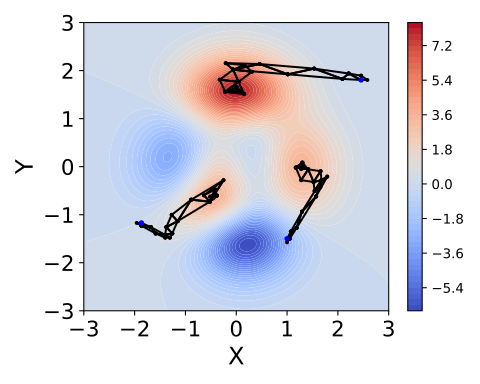
\includegraphics[height=3.2cm]{images/part1/opt/example_nelder_mead.png}
\caption{}
\labelsyn{fig:syn_ru:opt:opt_example_nelder_mead}
\end{subfigure}%
\begin{subfigure}[b]{.33\linewidth}
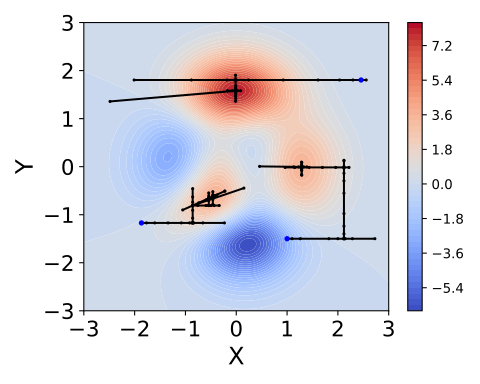
\includegraphics[height=3.2cm]{images/part1/opt/example_powell.png}
\caption{}
\labelsyn{fig:syn_ru:opt:opt_example_powell}
\end{subfigure}
\caption{Examples of local optimization methods applied to maximize the function shown in panel (a): (b) BFGS method, (c) Nelder-Mead method, (d) Powell method.}
\labelsyn{fig:syn_ru:opt:opt_example}
\end{figure}

Existing methods for selection of the best demographic model are described in \textbf{Section 1.6} alongside with modified approaches for model comparison.
At the beginning of the research in 2017, there was no method available for automatic model selection for demographic inference.
All model comparisons were performed manually by users using the Akaike information criterion or likelihood ratio test.
A single software tool~\cite{rippe2021environmental} implementing an alternative automatic model selection method became available after the publication of the first article of this dissertation~\cite{noskova2020gadma}.
However, it is limited to the analysis of two populations and assumes data independence.
In general, genetic data contain dependencies, as certain genomic regions are inherited together.
The Akaike information criterion and likelihood ratio test incorrectly favor models with more parameters when the data is dependent~\cite{gao2010composite}.
Existing modifications of these criteria~\cite{coffman2016computationally} account for these dependencies.

\underline{\textbf{Chapter 2}} describes the developed class of extended demographic models, two methods for parameter tuning using a combination of global and local optimization methods, and experimental studies of the developed models and methods.

\textbf{Section 2.1} provides a description of the developed class of extended demographic models, its implementation, and usage examples.
The first class of models was used as a prototype of the class of extended models.
The proposed extended models include a new type of parameters for tuning, which are discrete parameters representing one of three dependencies: constant population size, linear change, or exponential change.
The representation of the proposed model and the demographic histories for different parameter values (\texttt{Dyn}) are shown in Figure~\ref{fig:new_model:model}.

\begin{figure}[ht]
\centering
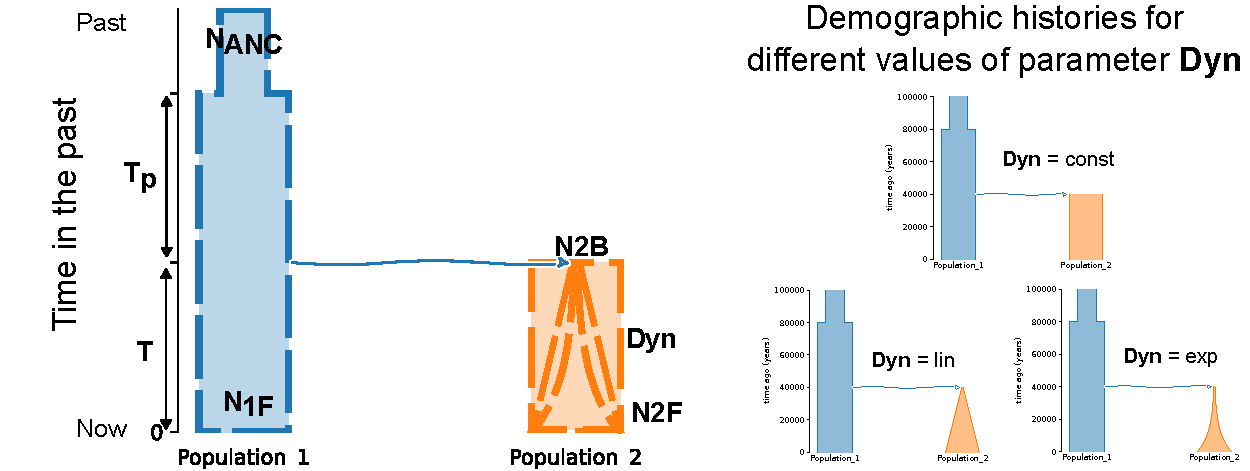
\includegraphics[width=0.9\linewidth]{images_2/picture_2pops_model_3_en.pdf}
\caption{Example of an extended demographic model for two populations and the corresponding demographic histories for different values of the parameter \texttt{Dyn}}
\labelsyn{fig:new_model:model}
\end{figure}

The formal description of the first proposed method for parameters tuning of the extended models in \textbf{Section 2.2}.
It is based on a combination of a genetic algorithm and local search is presented.
The section includes the description of the general scheme of method, the operators of mutation and crossover in the genetic algorithm.
The implementation details, and examples of applying the proposed method are also included.
Additionally, the section presents the results of hyperparameter tuning of the genetic algorithm that was performed to increase efficiency of the method.

\textbf{Section 2.3} describes the second developed method for parameter tuning of extended models, that is based on a combination of Bayesian optimization and local search.
The description of Bayesian optimization and its components, an existing cross-validation method for hyperparameter selection, and the implementation of the developed method are provided.
Similar to the genetic algorithm, hyperparameters of Bayesian optimization are tuned.
Based on conducted experimental studies for manual tuning, an ensemble Bayesian optimization approach was proposed.

\textbf{Section 2.4} includes conducted experimental studies of the developed method for parameter tuning that is based on a combination of a genetic algorithm and local search.

First, experimental studies of the developed method in combination with the likelihood computation method implemented in \textit{moments} are conducted.
A comparison is made between the developed method and the Powell method with restarts and the sequential runs of the Nelder-Mead method implemented in \textit{moments-pipeline}.
Models from the first class and three sets of simulated data are used for comparison.
The comparison shows that the developed method (GA) allows for more effective parameter tuning of models (Table~\ref{tab:part2:experiments:simulated_3:results}).
Furthermore, the proposed extended models are considered, and their parameters are tuned using the developed method.
The method correctly finds the parameters of the extended models, including the dynamics of population size changes.

\begin{table}[bh!]
\caption{Results of experimental studies for comparing parameter tuning methods on simulated data of three populations}
\resizebox{\linewidth}{!}{
\begin{tabular}{|l | c | c | c |}
\hline
& Powell's method & \multirow{2}{*}{\textit{moments-pipeline}} & \multirow{2}{*}{GA}\\
& with restarts & & \\
\hline
Mean number of likelihood evaluations & $22{,}475$ & $19{,}452$ & $21{,}651$ \\
\hline
Mean $f^{\text{\moments}}$ &$-11{,}178.62$ & $-11{,}179.82$ & $\mathbf{-11{,}178.45}$\\
\hline
Standard deviation of $f^{moments}$ & $0.40$ & $0.72$ & $\mathbf{0.15}$\\
\hline
Best $f^{\text{\moments}}$ & $-11{,}178.31$ & $-11{,}178.59$ & $\mathbf{-11{,}178.29}$\\
\hline
\end{tabular}%
}
\labelsyn{tab:part2:experiments:simulated_3:results}
\end{table}

Next, three experimental studies of the developed method in combination with the likelihood computation method implemented in \dadi are conducted.

The method is applied to real data of Gaboon forest frog (\textit{Scotobleps gabonicus}), previously analyzed in~\cite{portik2017evaluating} using \textit{dadi-pipeline}.
Demographic histories for three different pairs of populations are obtained using the same 12 models used in~\cite{portik2017evaluating}.
For 92\% of the models, the developed method finds parameters with higher likelihood values compared to those obtained using \textit{dadi-pipeline}.
In 5\% of cases, the likelihood values are the same, and only for one model (3\%) it is worse.

On data of two puma populations (\textit{Puma concolor}), the developed method is compared to the BFGS method with restarts and the BOBYQA method with restarts.
Two models, proposed and analyzed previously in~\cite{blischak2020inferring}, without and with inbreeding, are used.
The results show that the developed method, on average, outperforms the BFGS and BOBYQA methods (Table~\ref{tab:part2:experiments:puma:puma_F_res}).
Additional parameter tuning using an extended parameter bounds provides a demographic history with a higher likelihood value than previously achieved.

\begin{table}[ht]
    \centering
    \caption{Results of 100 repeats of different methods for parameter tuning in case of model 2 with inbreeding for two puma populations}
    \resizebox{\linewidth}{!}{%
    \begin{tabular}{|p{3.3cm}|P{1.9cm}|P{1.9cm}|P{1.9cm}|P{1.9cm}|P{1.9cm}|}
         \hline
         & \multicolumn{2}{c|}{BFGS} &  \multicolumn{2}{c|}{BOBYQA} & GA \\
         &  1 restart & 16 restarts & 1 restart & 4 restarts &\\
         \hline
         Number of likelihood evaluations & $394\pm82$ & $6{,}245\pm324$ & $1{,}605 \pm 1{,}207$ & $6{,}095 \pm 2{,}561$ & $6{,}193\pm2{,}680$ \\
         \hline
         Time CPU (min) &  $1.3\pm1.4$ & $25\pm19$ & $ 12\pm 5$ & $16\pm7$ & $93\pm47$ \\
         \hline
         Best likelihood &  $-317{,}370.88$ & $-317{,}370.88$ & $\mathbf{-317{,}239.48}$ & $\mathbf{-317{,}239.48}$ & $-317{,}239.49$ \\
         \hline
         Mean likelihood &  $-1{,}729{,}870$ & $-320{,}947$ & $-381{,}979$ & $-320{,}503$ & $\mathbf{-319{,}451}$ \\
         \hline
         Standard deviation & $4{,}339{,}276$ & $5{,}029$ & $115{,}205$ & $8{,}753$ & $7{,}340$ \\
         \hline
    \end{tabular}%
    }
    \labelsyn{tab:part2:experiments:puma:puma_F_res}
\end{table}

Similarly, the developed method is compared to the BOBYQA method with restarts on domestic cabbage data (\textit{Brassica oleracea}), previously analyzed in~\cite{blischak2020inferring}.
On these data, the BOBYQA method with multiple restarts shows better results than the developed method.
However, it should be noted that the number of restarts required for the BOBYQA method to achieve this efficiency is unknown in general.
The demographic inference with extended parameter bounds provides histories with higher likelihood values than before.

Then, four existing likelihood computation methods implemented in \dadi, \moments, \momi, and \momentsLD, are compared using the developed method on orangutan data simulated using the \textit{stdpopsim} library~\cite{adrion2020community,lauterbur2023expanding}.
The comparison is made using different models, including extended models from the proposed class.
It is shown that all methods are able to recover the true demographic history when correct models are used.
Using misspecified models, that could not capture the true history, such as models without continuous migrations, leads to differences in the obtained results (Figure~\ref{fig:part2:experiments:sim2:results:oran_momi}).
However, it should be noted that key population characteristics, such as population size, are properly found even in such cases.

\begin{figure}[ht]
    \centering
    \begin{subfigure}[b]{0.24\linewidth}
        \centering
        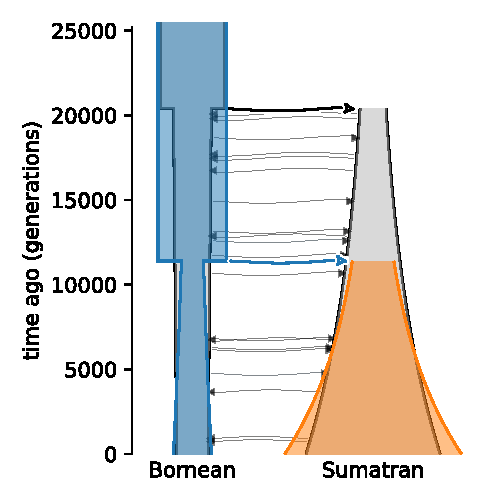
\includegraphics[width=\textwidth]{images_experiments/suimulation_2_stdpopsim/ORAN-PULSE/oran-nomig.pdf}
        \caption{}
        \labelsyn{fig:part2:experiments:sim2:results:oran_momi_nomig}
    \end{subfigure}%
    \begin{subfigure}[b]{0.24\linewidth}
        \centering
        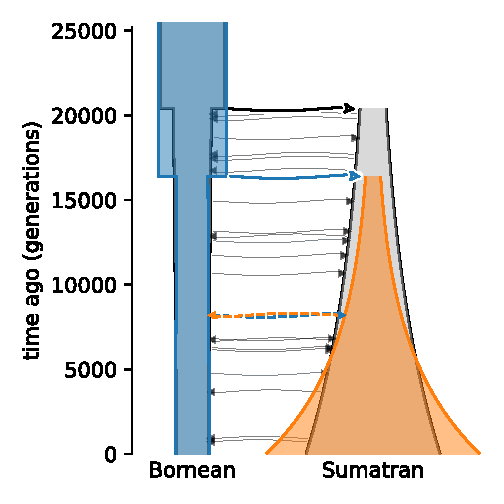
\includegraphics[width=\textwidth]{images_experiments/suimulation_2_stdpopsim/ORAN-PULSE/oran-pulse-1.pdf}
        \caption{}
        \labelsyn{fig:part2:experiments:sim2:results:oran_pulse_1}
    \end{subfigure}%
    \begin{subfigure}[b]{0.24\linewidth}
        \centering
        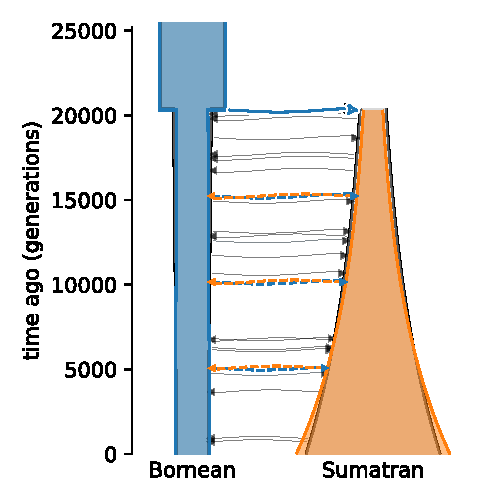
\includegraphics[width=\textwidth]{images_experiments/suimulation_2_stdpopsim/ORAN-PULSE/oran-pulse-3.pdf}
        \caption{}
        \labelsyn{fig:part2:experiments:sim2:results:oran_pulse_3}
    \end{subfigure}%
    \begin{subfigure}[b]{0.24\linewidth}
        \centering
        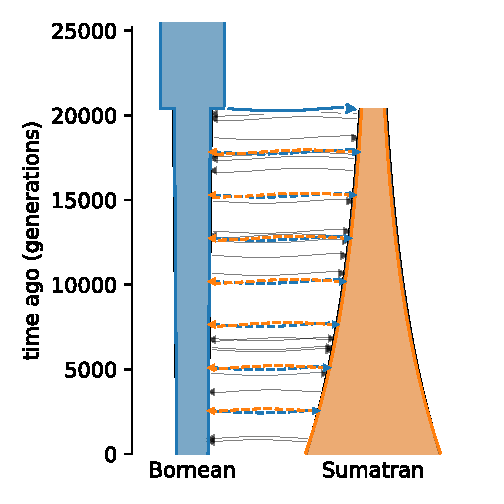
\includegraphics[width=\textwidth]{images_experiments/suimulation_2_stdpopsim/ORAN-PULSE/oran-pulse-7.pdf}
        \caption{}
        \labelsyn{fig:part2:experiments:sim2:results:oran_pulse_7}
    \end{subfigure}
    \caption{Results of tuned models for the likelihood computation method implemented in \momi (a)~model without migrations, and models with (b)~one, (c)~three, (d)~seven pulse migrations}
    \labelsyn{fig:part2:experiments:sim2:results:oran_momi}
\end{figure}

Finally, the demographic history of three populations of modern humans in Russia is inferred: the inhabitants of Pskov, Novgorod, and Yakutia.
The data used in this analysis has not been previously analyzed.
The parameters of the extended model are tuned using the developed method based on the combination of genetic algorithm and local search.
The obtained demographic history (Figure~\ref{fig:part2:experiments:rus:result}) is consistent with the known history of modern humans~\cite{schraiber2015methods, nielsen2017tracing}.

\begin{figure}[ht]
\centering
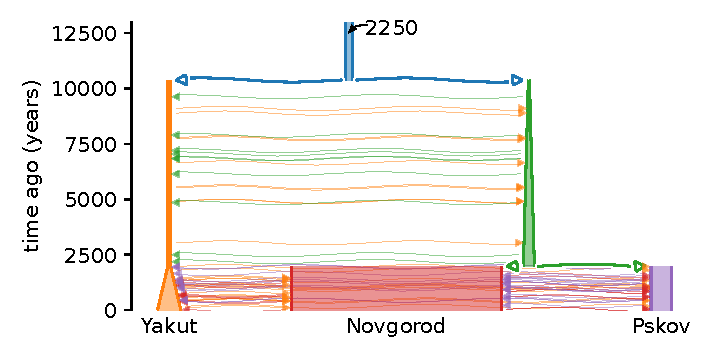
\includegraphics[width=0.8\linewidth]{images_experiments/rus_genomes/picture_result.pdf}
\caption{Obtained demographic history of three populations of modern humans}
\labelsyn{fig:part2:experiments:rus:result}
\end{figure}

\textbf{Section 2.5} describes the results of conducted experimental studies of the developed method for parameter tuning, that is based on the combination of Bayesian optimization and local search.

Bayesian optimization is compared to the genetic algorithm on a set of datasets (Figure~\ref{fig:bo_ga_comp}).
It was shown that the genetic algorithm (GA) is more efficient in the case of one, two, and three populations.
Bayesian optimization (BO) has faster convergence than the genetic algorithm when considering more than three populations.
Applying Bayesian optimization allows reducing the time required for parameter tuning by 50-80\% which leads to significant acceleration of the process by days and even by weeks.


\begin{figure}[ht]
\centering
\begin{subfigure}[b]{0.49\linewidth}
\centering
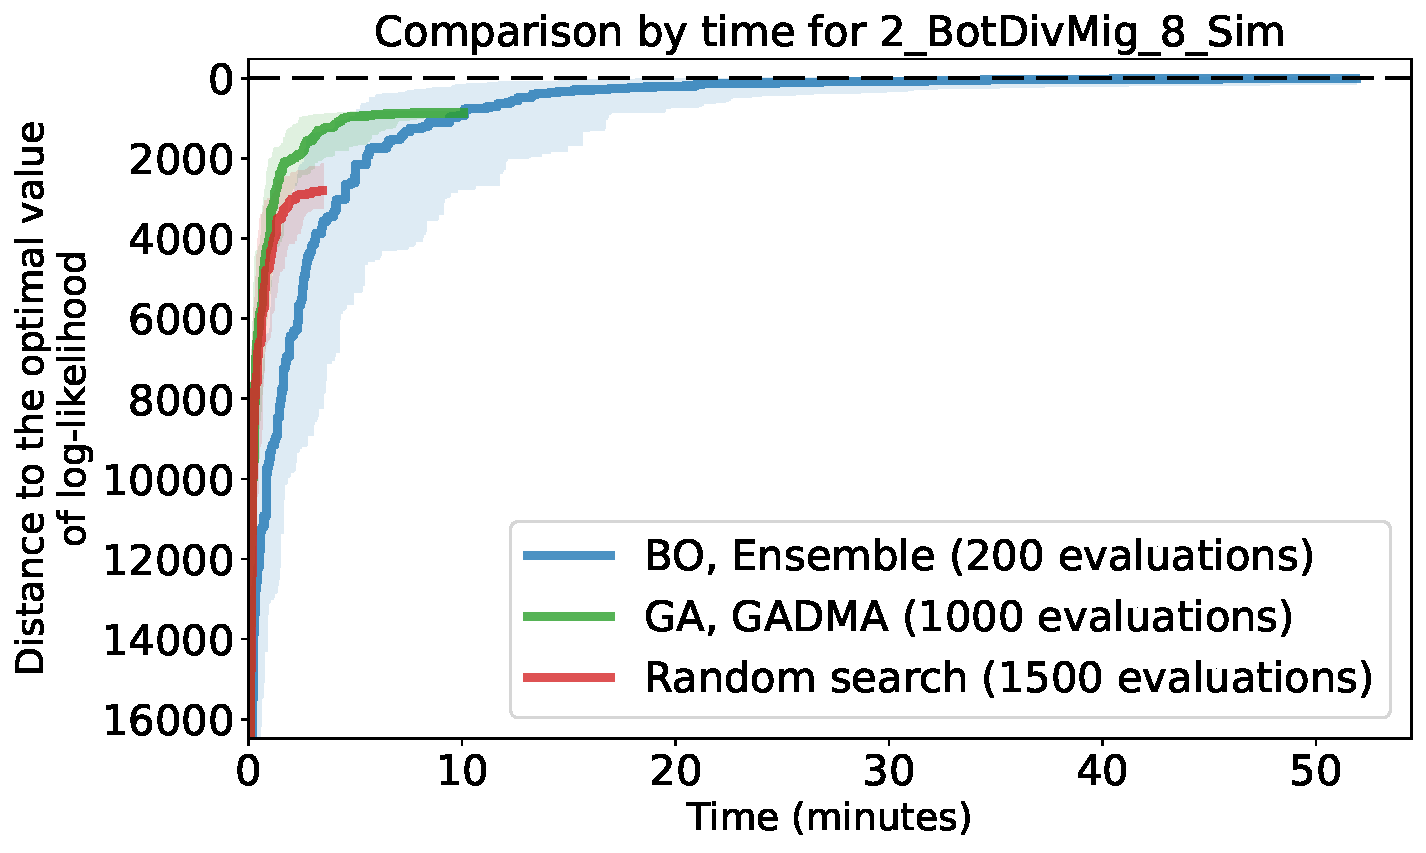
\includegraphics[width=0.9\textwidth]{images_experiments/bo_ga/2_BotDivMig_8_Sim_bo_ga_time.pdf}
\caption{}
\labelsyn{fig:bo_ga_comp:2pops}
\end{subfigure}%
\begin{subfigure}[b]{0.49\linewidth}
\centering
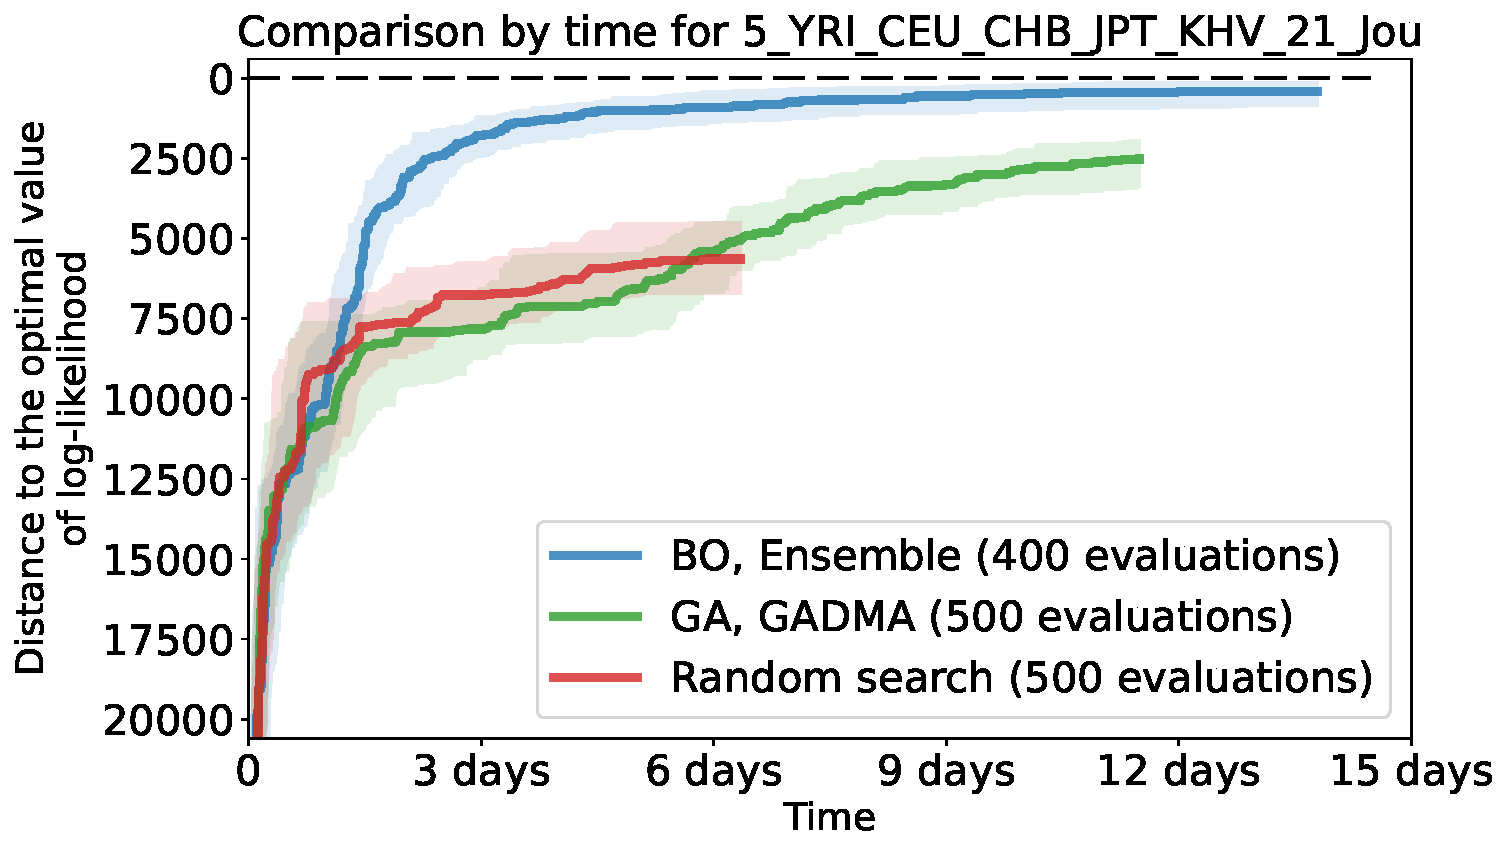
\includegraphics[width=0.9\textwidth]{images_experiments/bo_ga/5_YRI_CEU_CHB_JPT_KHV_21_Jou_bo_ga_time.pdf}
\caption{}
\labelsyn{fig:bo_ga_comp:5pops}
\end{subfigure}
\caption{Convergence over time of parameter tuning methods for (a) two populations, (b) five populations.}
\labelsyn{fig:bo_ga_comp}
\end{figure}

Furthermore, the developed method based on the combination of Bayesian optimization and local search is used to tune the parameters of demographic models for four and five populations using real data of modern humans from~\cite{jouganous2017inferring}.
The developed method allows obtaining parameters that yielded a higher likelihood than those found in~\cite{jouganous2017inferring} using the Powell's method with restarts.
Figure~\ref{fig:syn_ru:bo_human} demonstrates a comparison between the resulting demographic history with a higher likelihood and the history obtained in the original study.

\begin{figure}[t]
\centering
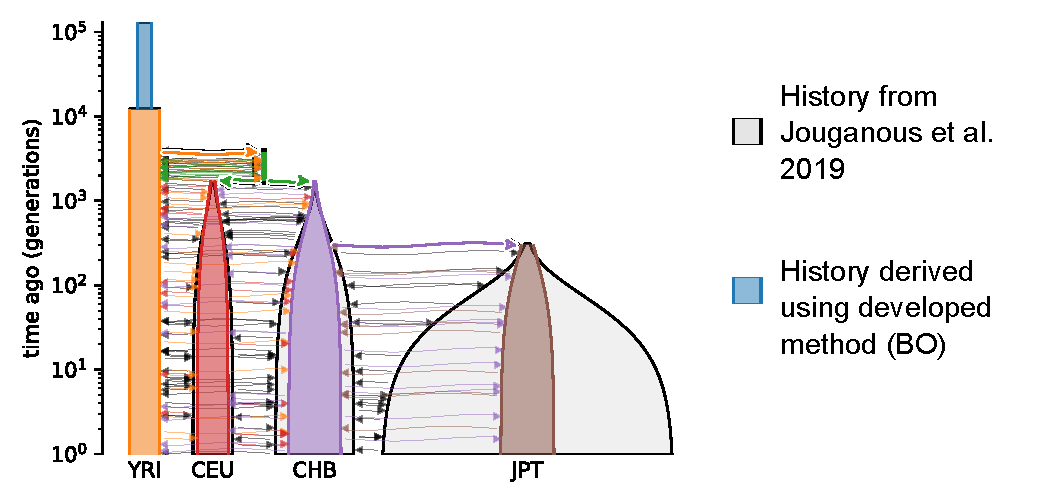
\includegraphics[width=0.8\linewidth]{images_experiments/bo_human/4pops_result_en.pdf}
\caption{Comparison of the demographic history obtained using the developed method (BO) and the demographic history from~\cite{jouganous2017inferring}.}
\labelsyn{fig:syn_ru:bo_human}
\end{figure}

The developed method of automatic model selection for demographic inference of one, two, and three populations is described in the \underline{\textbf{third chapter}}, along with the results of its application in combination with the developed method based on a genetic algorithm.

A formal description of the developed method is provided in \textbf{Section 3.1}.
The method takes the minimum and maximum constraints on the model as input.
In the first round, the method constructs a model that satisfies the minimum constraint and performs parameter tuning using the developed genetic algorithm-based method.
In each next round, the model is modified, the number of parameters is increased, and a new set of parameters is tuned. 
The method stops when the model reaches the maximum constraints.
Finally, all explored models are compared using the Akaike information criterion, and the best model is selected.
The number of time intervals in the model is proposed as the constraint for the models.



\textbf{Section 3.2} includes experimental studies of the developed automatic model selection method.
The demographic history of the «Out of Africa» scenario for genetic data of three modern human populations is obtained, as shown in Figure~\ref{fig:part4:experiments:3pop_human:result}. The result is consistent with other studies~\cite{gutenkunst2009inferring, schraiber2015methods, nielsen2007recent}.
It has not only a higher likelihood value than the history obtained in~\cite{gutenkunst2009inferring} using the same data, but also is better according to the Akaike information criterion.

\begin{figure}[t]
    \centering
        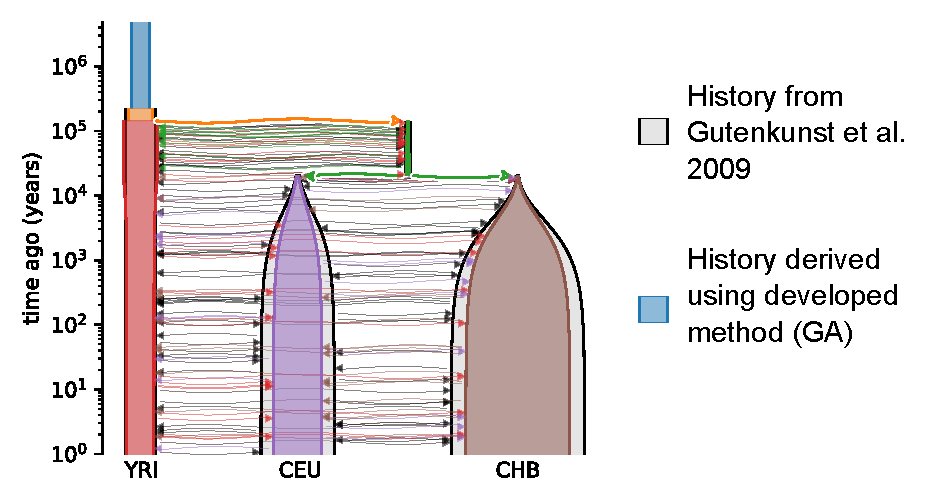
\includegraphics[width=0.8\textwidth]{images_experiments/3pop_human_gutenkunst/picture_3pop_result_en.pdf}
    \caption{Demographic history obtained by the developed method}
    \labelsyn{fig:part4:experiments:3pop_human:result}
\end{figure}

The automatic model selection method was applied to the real data of the Gaboon forest frog (\textit{Scotobleps gabonicus}).
Models for three different pairs of populations were constructed in Section 2.4 using manual brute force.
The models obtained through the automatic selection method exhibited the best Akaike information criterion values among all the configurations considered for two out of three population pairs.
In the case of the third population pair, the obtained model had a worse Akaike information criterion value compared to the best model obtained through manual brute force.
However, the results allow identifying a redundant model parameter, and excluding this parameter from the configuration resulted in the best Akaike information criterion value.

The developed method of automatic selection of extended models is used to infer the demographic history of blue shark populations.
The genetic data was not previously analyzed.
A sequential approach to inferring the demographic history of two and three populations is developed, resulting in the demographic history shown in Figure~\ref{fig:part2:experiments:blue_shark:3pop_hist}.
The inferred population sizes are consistent with other studies~\cite{king2015genetic,verissimo2017world}.
Validation of the results by colleagues in the field of zoology suggests that the split between the northern and southern populations of blue shark occurred in connection with paleoclimatic events during the Holocene epoch~\cite{leduc2010holocene,masson2013information,olsen2012variability}.

\begin{figure}[b]
    \centering
        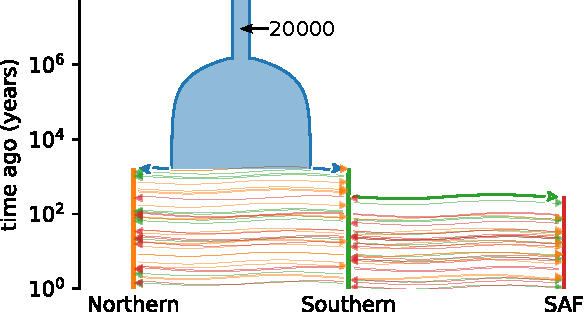
\includegraphics[width=0.6\linewidth]{images_experiments/blue_shark/3pop_history.pdf}
    \caption{Demographic history of three blue shark populations}
    \labelsyn{fig:part2:experiments:blue_shark:3pop_hist}
\end{figure}

The description of the software tools that implement the developed methods or are used in this work is provided in the \underline{\textbf{fourth chapter}}.

\textbf{Section 4.1} contains a description of the GADMA (Global Search Algorithm for Demographic Model Analysis) software framework, which implements the developed class of extended models, parameter tuning methods, and automatic mdoel selection method.
The structure of the software package is shown in Figure~\ref{fig:syn_ru:gadma_modules}.

\begin{figure}[ht]
\centering
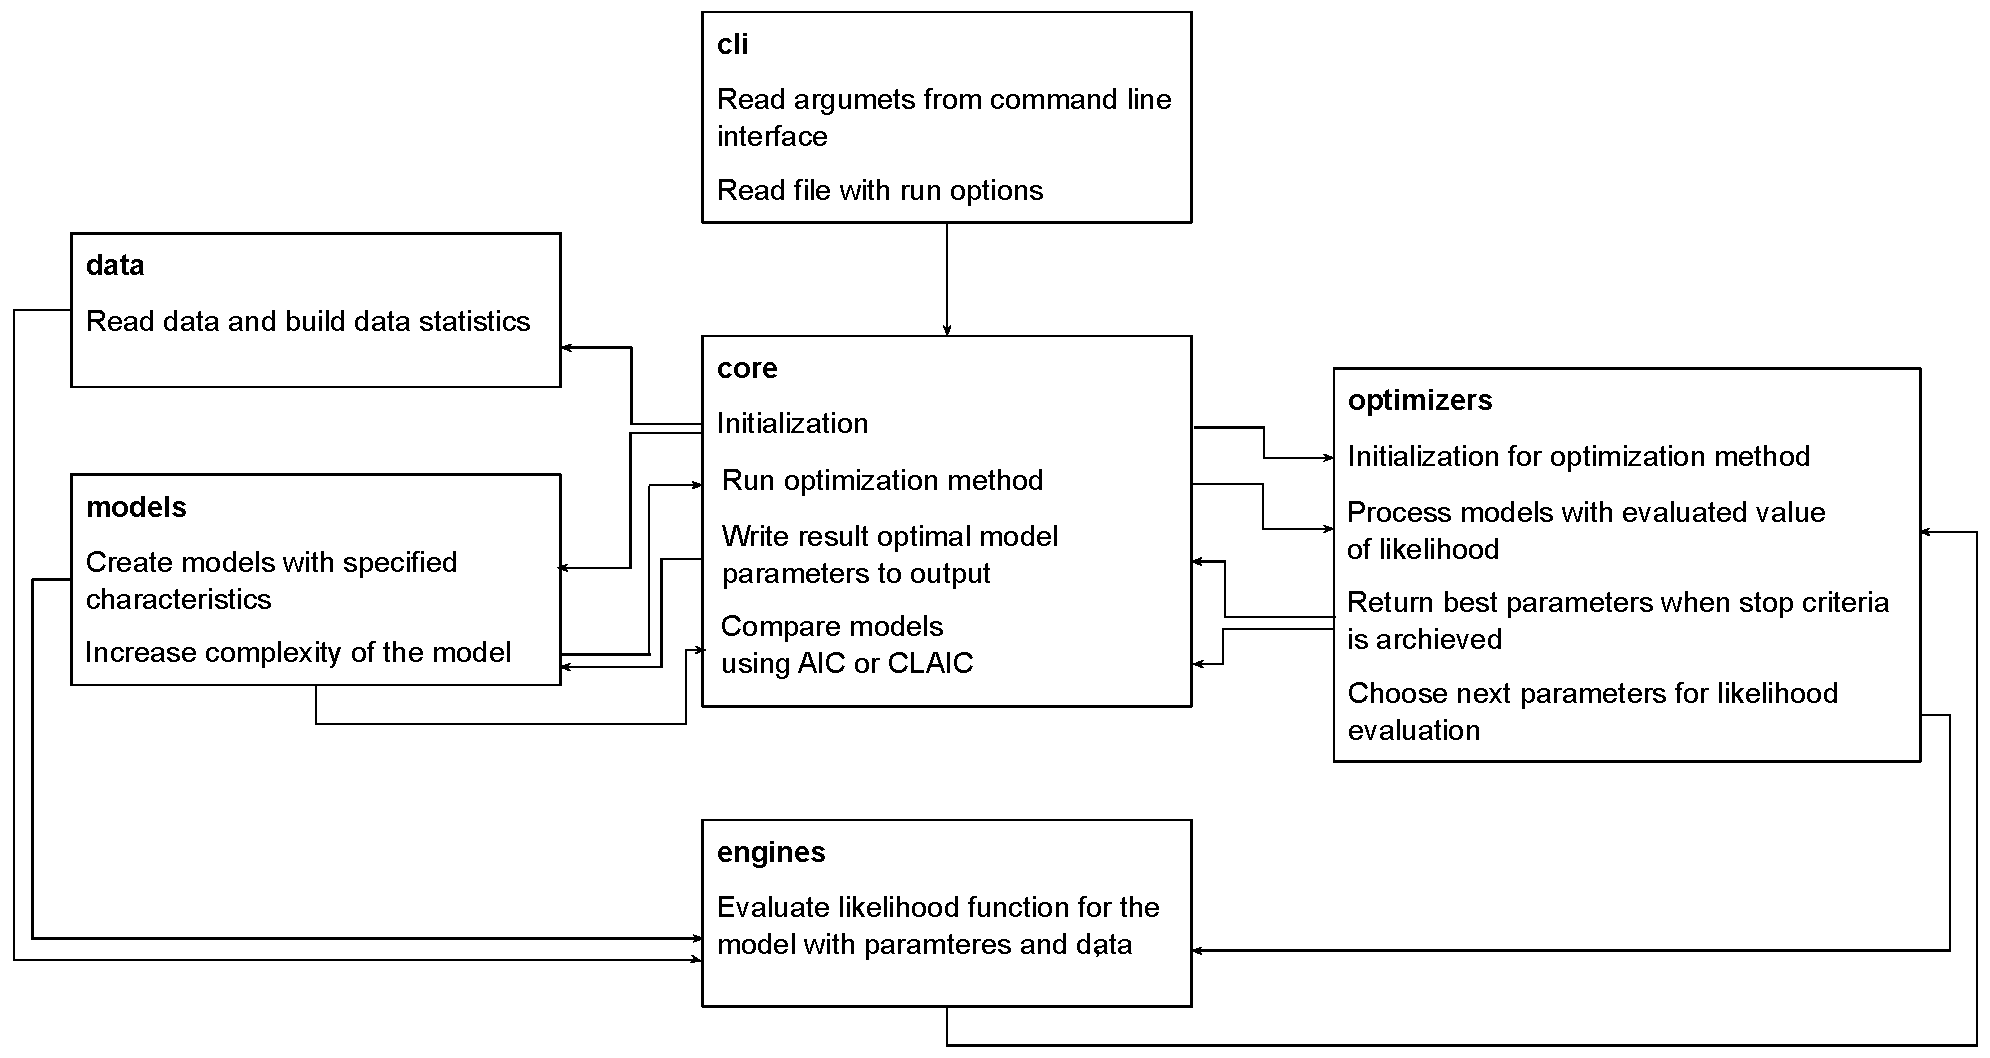
\includegraphics[width=\linewidth]{images/part5/gadma_modules_en.pdf}
\caption{Structure of the GADMA software framework.}
\labelsyn{fig:syn_ru:gadma_modules}
\end{figure}

The extension of the \textit{stdpopsim} and \textit{demes} libraries is described in \textbf{Section 4.2}.
The \textit{stdpopsim} library provides a catalog of predefined species and their demographic histories for more reliable genetic data simulations.
This library was extended and used in the experimental studies.
The \textit{demes} software is designed for textual and visual representation of demographic histories.
This library is extended with the implementation of linear population size changes and is integrated into the GADMA software framework.
All the visualizations of demographic histories in this thesis are obtained using the \textit{demes} library.

To \textbf{conclude}, the results of this study are:

%!TEX root = ../dissertation.tex
\begin{itemize}
    \item The current state of the research field has been investigated, clarifying the problem and methods for evaluating results;
    \item The formalization of the problem of building and tuning models of metric trees with functions on edges considered on the example of the demographic inference from genetic data.
    \item The method for automatic tuning of the models of metric trees with functions on edges based on a combination of global and local optimization methods was developed considered on the example of the demographic inference from genetic data;
    \item The method for automatic selection of model of metric tree with functions on edges was developed considered on the example of the demographic inference from genetic data;
    \item The software package that incorporates the developed models and methods for inferring the demographic history of populations from genetic data was designed and implemented;
    \item experimental studies confirming the effectiveness of the developed models and methods, as well as their applicability for inferring the demographic history of populations from genetic data were carried out, and the results of the experiments were analyzed.\\
\end{itemize}

The value of the likelihood function was used to evaluate the quality of demographic history models in this work.
Experimental results show that the method of model parameter tuning based on a combination of genetic algorithm and local search allowed to find model parameters that provide a better likelihood value in 88\% of cases (37 models out of 42 tested) than the parameters found by existing methods.
Using simulated data, the developed method allowed us to find solutions that are 97\% closer to the optimum in the case of one population and 66\% closer to the optimum in the case of three populations than the solutions obtained by existing methods.
The tuning of the hyperparameters of the genetic algorithm allowed to speed up the implementation by 10\% on average while maintaining the efficiency of the method.

The effectiveness of the method for tuning model parameters based on Bayesian optimization and local optimization under conditions of a computationally complex target function was confirmed.
The developed method made it possible to find parameter values providing a better likelihood value than existing methods for two previously analyzed data of four and five populations.
It was shown that Bayesian optimization achieves a solution close to the optimum 50-80\% faster than the genetic algorithm in the case of inferring the demographic history of four and five populations.

The method of automatic model selection allows to automatically build and tune models within given configuration constraints.
The comparison of models of demographic histories with different numbers of parameters was performed using the Akaike Information Criterion (AIC).
Experimental studies showed that in three out of four cases, the method was able to find a model that provided a better AIC value than was previously obtained by manual brute force.
In the fourth case, the resulting model allowed to identify a redundant parameter in the configuration and build a nested model that finally provided the best AIC value for the data.

As promising areas of research we can highlight the improvement of the method of automatic model selection in order to find the optimal set of configuration parameters, as well as the development of methods for tuning metric tree models with functions on the edges, which allow not only the tuning of functional parameters, but also the search for the optimal tree structure.
